% ICSE 2027 Industry Challenge, Solution Paper for Challenge #2.
% Format per CFP: IEEE conference template, 10pt, no compsoc options.
% Limit: 10 pages including figures, tables and appendices, plus up to
% 2 pages containing only references. Double-anonymous.
\documentclass[10pt,conference]{IEEEtran}

\usepackage[T1]{fontenc}
\usepackage{amsmath,amssymb}
\usepackage{cite}
%% \PassOptionsToPackage{hidelinks,unicode}{hyperref} % Example options

%%%%%%%%% PACKAGES

\usepackage{booktabs}     % for nice horizontal lines
%\usepackage{caption}

% --- Preamble (place in your preamble) ---
% \usepackage[switch]{lineno} 
\usepackage{graphicx}
% \usepackage{subcaption} % disabled: caption package overrides IEEEtran captions (see NOTES.md N45)
\usepackage{placeins} % for \FloatBarrier to control float placement
\usepackage{float}     % for [H] exact float placement
% Independent "Listing N" float with a two-column (starred) variant for the
% motivating-example diff. newfloat only needs keyval, so it does not pull in
% the caption package (which conflicts with acmart).
\usepackage{newfloat}
\DeclareFloatingEnvironment[name=Listing, fileext=lol, placement=tbp, within=none]{listing}
\usepackage{tcolorbox}
\tcbuselibrary{skins,breakable,listings}
\usepackage{listings}
\usepackage{xcolor}  % table option passed via \PassOptionsToPackage in main.tex
\usepackage{array}
% Listings styles
\lstdefinestyle{code}{
  basicstyle=\ttfamily\small,
  numbers=left, numberstyle=\scriptsize, numbersep=6pt,
  breaklines=true, breakatwhitespace=true,
  frame=single, framerule=0.4pt,
  tabsize=2, showstringspaces=false
}
\lstdefinestyle{cpp}{style=code, language=C++}
\lstdefinestyle{json}{style=code, language=}
\lstdefinestyle{txt}{style=code, language=}

% Ensure circled step numbers in listings render reliably
% Maps Unicode circled digits to the TikZ-based \circled{n} macro
\lstset{literate=
  {❶}{{\circled{1}}}1
  {❷}{{\circled{2}}}1
  {❸}{{\circled{3}}}1
  {❹}{{\circled{4}}}1
  {❺}{{\circled{5}}}1
  {❻}{{\circled{6}}}1
  {❼}{{\circled{7}}}1
}

% A reusable “code card” environment
\newtcblisting{codecard}[2][]{%
  enhanced, breakable,
  colback=white, colframe=black!12,
  boxrule=0.6pt, arc=2mm, left=1mm, right=1mm, top=1mm, bottom=1mm,
  title={#2}, fonttitle=\bfseries\footnotesize,
  listing only, listing options={#1}
}

% --- GitHub-style split-diff support (used in the Motivating Example) ---------
% Per-cell background highlighting via colortbl's \cellcolor (loaded explicitly
% here: the class loads xcolor *without* the table option, so \cellcolor/\rowcolor
% are otherwise undefined). Code is typeset with \lstinline so quotes/brackets
% stay verbatim-safe.
\usepackage{colortbl}
\definecolor{diffadd}{RGB}{225,251,231}   % GitHub-ish light green (added)
\definecolor{diffdel}{RGB}{255,233,232}   % GitHub-ish light red   (removed)
% Minimal Swift language (listings has no built-in Swift definition)
\lstdefinelanguage{Swift}{%
  morekeywords={func,let,var,while,for,in,if,else,guard,return,true,false,nil},
  sensitive=true, morestring=[b]", morecomment=[l]{//}}
% Compact inline style for the diff cells; long UI-locator lines need it small.
\lstdefinestyle{swiftmini}{%
  basicstyle=\ttfamily\scriptsize, columns=fullflexible, keepspaces=true,
  language=Swift, keywordstyle=\bfseries\color{blue!60!black},
  literate={"}{{\textquotedbl}}1}
% +/- gutter glyphs and the gray line-number cell
\newcommand{\gplus}{\textcolor{green!55!black}{\ttfamily\scriptsize +}}
\newcommand{\gminus}{\textcolor{red!70!black}{\ttfamily\scriptsize $-$}}
\newcommand{\dnum}[1]{\textcolor{black!40}{\ttfamily\scriptsize #1}}
% Shorthand: shade the three cells of one diff half-row (color, then lineno/gutter/code)
\newcommand{\dadd}{\cellcolor{diffadd}}
\newcommand{\ddel}{\cellcolor{diffdel}}
% Code cell + keyword: \lstinline cannot be used here because colortbl/array
% re-scans cells and breaks its verbatim catcodes, so we typeset code as plain
% monospace (T1 renders ", [, ], <, > correctly; ~ gives visible indentation).
\newcommand{\cd}[1]{{\ttfamily\scriptsize\strut #1}}
\newcommand{\kw}[1]{\textcolor{blue!60!black}{\textbf{#1}}}
% One full diff line in a single (optionally shaded) cell, so the line number,
% the +/- gutter, and the code share one continuous background. Fixed-width
% \makebox keeps the columns aligned and guarantees the gap after the number.
% #1=row color, #2=line number, #3=gutter glyph (\gplus/\gminus or empty), #4=code
\newcommand{\diffline}[4]{%
  \cellcolor{#1}\makebox[1.3em][r]{\dnum{#2}}\hspace{8pt}%
  \makebox[0.6em][c]{#3}\hspace{6pt}\cd{#4}}



%% \usepackage{soul}
% xcolor is loaded by the class with the 'table' option (now explicitly loaded above)
\usepackage{tabularx}
%% %% Custom packages end here

%% \usepackage{cite}
%% \usepackage{amsmath}
%% \usepackage{booktabs}
\usepackage{wrapfig}
\usepackage{multirow}
\usepackage{multicol}
\usepackage{enumitem}
%% \usepackage{color}
\usepackage{listings}
%% \usepackage{graphicx}
%% \usepackage{rotate}
%% %% \usepackage{url}
%% %\usepackage[hidelinks]{hyperref}
%% \usepackage{breakurl}
%% \usepackage{flushend}
\usepackage{xspace}
%% \usepackage[round-mode=places,round-precision=1,group-separator={,},group-minimum-digits={3},output-decimal-marker={.}, round-pad=false, exponent-mode = threshold, exponent-thresholds = -3:5, tight-spacing=true]{siunitx}
% \usepackage{subcaption} % disabled: caption package overrides IEEEtran captions (see NOTES.md N45)
%\usepackage{pgf-pie}
%% \usepackage{bbding}
\usepackage{pifont}
%% \usepackage{seqsplit}
%% \usepackage{pgfplots}
%% \pgfplotsset{width=7cm,compat=1.8}
%% \usepackage{datetime2}

%% % Tikz Figs
\usepackage{tikz}
\tikzset{>=latex}
\usetikzlibrary{shapes.geometric,arrows.meta,positioning,fit,backgrounds,calc} % for flow diagrams and icon pics

%%%%%%%%%
% ---------- Icon pics (line-art, ~0.5 cm) ----------
\tikzset{
  ic/.style={line width=0.6pt, line cap=round, line join=round},
  pics/play/.style={code={
    \draw[ic] (0,0) circle (0.26);
    \fill (-0.08,-0.13) -- (-0.08,0.13) -- (0.16,0) -- cycle;
  }},
  pics/search/.style={code={
    \draw[ic] (0.03,0.06) circle (0.16);
    \draw[ic] (-0.09,-0.06) -- (-0.22,-0.19);
  }},
  pics/bug/.style={code={
    \draw[ic] (0,0) ellipse (0.15 and 0.21);
    \draw[ic] (0,0.21) -- (0,0.30);
    \draw[ic] (0,0.30) circle (0.07);
    \draw[ic] (-0.04,0.36) -- (-0.09,0.43);
    \draw[ic] (0.04,0.36) -- (0.09,0.43);
    \foreach \y in {0.10,0,-0.10}{
      \draw[ic] (-0.13,\y) -- (-0.26,\y+0.05);
      \draw[ic] (0.13,\y) -- (0.26,\y+0.05);
    }
  }},
  pics/shield/.style={code={
    \draw[ic] (0,0.24) -- (-0.17,0.17) -- (-0.17,-0.07)
      .. controls (-0.17,-0.20) and (-0.07,-0.28) .. (0,-0.30)
      .. controls (0.07,-0.28) and (0.17,-0.20) .. (0.17,-0.07)
      -- (0.17,0.17) -- cycle;
    \draw[ic] (-0.08,0.0) -- (-0.02,-0.08) -- (0.10,0.10);
  }},
  pics/funnel/.style={code={
    \draw[ic] (-0.22,0.20) -- (0.22,0.20) -- (0.05,-0.05) -- (0.05,-0.22)
      -- (-0.05,-0.22) -- (-0.05,-0.05) -- cycle;
  }},
  pics/db/.style={code={
    \draw[ic] (-0.16,0.18) arc (180:360:0.16 and 0.07);
    \draw[ic] (-0.16,0.18) arc (180:0:0.16 and 0.07);
    \draw[ic] (-0.16,0.18) -- (-0.16,-0.18);
    \draw[ic] (0.16,0.18) -- (0.16,-0.18);
    \draw[ic] (-0.16,0.0) arc (180:360:0.16 and 0.07);
    \draw[ic] (-0.16,-0.18) arc (180:360:0.16 and 0.07);
  }},
  pics/brain/.style={code={
    \draw[ic] (0,0.26)
      .. controls (-0.22,0.26) and (-0.28,0.08) .. (-0.20,-0.02)
      .. controls (-0.30,-0.10) and (-0.20,-0.28) .. (-0.05,-0.22)
      .. controls (0.0,-0.30) and (0.0,-0.30) .. (0.05,-0.22)
      .. controls (0.20,-0.28) and (0.30,-0.10) .. (0.20,-0.02)
      .. controls (0.28,0.08) and (0.22,0.26) .. (0,0.26) -- cycle;
    \draw[ic] (0,0.26) -- (0,-0.24);
    \draw[ic] (-0.10,0.12) .. controls (-0.02,0.10) and (-0.02,0.0) .. (-0.10,-0.04);
    \draw[ic] (0.10,0.12) .. controls (0.02,0.10) and (0.02,0.0) .. (0.10,-0.04);
  }},
  pics/book/.style={code={
    \draw[ic] (0,-0.16) .. controls (-0.10,-0.24) and (-0.24,-0.20) .. (-0.26,-0.16)
      -- (-0.26,0.16) .. controls (-0.20,0.12) and (-0.06,0.10) .. (0,0.18);
    \draw[ic] (0,-0.16) .. controls (0.10,-0.24) and (0.24,-0.20) .. (0.26,-0.16)
      -- (0.26,0.16) .. controls (0.20,0.12) and (0.06,0.10) .. (0,0.18);
    \draw[ic] (0,0.18) -- (0,-0.16);
  }},
  pics/graph/.style={code={
    \draw[ic] (-0.30,0) -- (0.30,0);
    \draw[ic] (0,0) -- (0,0.20);
    \foreach \x in {-0.30,-0.10,0.10,0.30}{ \fill (\x,0) circle (0.035); \draw[ic] (\x,0) circle (0.035);}
    \fill (0,0.20) circle (0.035); \draw[ic] (0,0.20) circle (0.035);
  }},
  pics/repo/.style={code={
    \draw[ic] (-0.10,0.26) -- (-0.10,-0.26);
    \foreach \y in {0.20,-0.04,-0.20}{ \fill (-0.10,\y) circle (0.05); \draw[ic](-0.10,\y) circle (0.05);}
    \draw[ic] (-0.10,-0.04) .. controls (0.06,-0.04) and (0.16,0.04) .. (0.16,0.16);
    \fill (0.16,0.20) circle (0.05); \draw[ic] (0.16,0.20) circle (0.05);
  }},
}
%%%%%%%%%


%% %\usepackage{pgf-umlsd} % for flow diagram
%% \usetikzlibrary{calc}
%% \usetikzlibrary{shapes.geometric}
%% \usetikzlibrary{decorations.pathreplacing}
%% \usetikzlibrary{positioning}
\newcommand*\circled[1]{\tikz[baseline=(char.base)]{
            \node[shape=circle,draw,fill=black,text=white,inner
            sep=0.4pt] (char) {\small #1};}}

%% %%%%%%%%%% CHECKMARKS


%% %%%%%%%% CONCLUDING BOXES
\usepackage[framemethod=tikz]{mdframed}
\mdfdefinestyle{mpdframe}{
   frametitlebackgroundcolor   =black!15,
    frametitlerule              =true,
    roundcorner                 =3pt,
    middlelinewidth             =1pt,
    skipabove                   =\topskip,
    skipbelow                   =\topskip,
    innermargin                 =0.1cm, % smaller makes box bigger
    outermargin                 =0.1cm,
    innerleftmargin             =0.1cm,
    innerrightmargin            =0cm,
    innertopmargin              =0.1cm,
    innerbottommargin           =0.1cm,
    align=center   
}

%%%%%%%%%% CODE and MACROS

%\input{defs-code}
%% \input{defs-logic}

%%%%%%%%%% UNCLASSIFIED
\newcommand{\Caption}[1]{\caption{#1}}
\newcommand{\NAtname}{-}
\newcommand{\specialcell}[2][c]{\begin{tabular}[#1]{@{}c@{}}#2\end{tabular}}
% Right-aligned special cell for numbers with inline deltas
\newcommand{\specialcellr}[1]{\begin{tabular}[c]{@{}r@{}}#1\end{tabular}}
\newcommand{\DefMacro}[2]{%
   \expandafter\newcommand\csname rmk-#1\endcsname{#2}%
}
\newcommand{\UseMacro}[1]{\csname rmk-#1\endcsname}


\newcommand{\YC}{\textcolor{blue}{\textbf{+}}} %{$\checkmark$}}
\newcommand{\NC}{\textcolor{red}{\textbf{-}}} %\textbf{$\times$}}}
\newcommand{\MC}{\textcolor{magenta}{\textbf{$\pm$}}}

\newcommand{\etal}{et al.}
\newcommand{\eg}{e.g.}
\newcommand{\ie}{i.e.}
\newcommand{\Fix}[1]{\textcolor{red}{[#1]}}
\newcommand{\Den}[1]{\textcolor{blue}{Denini:~[#1]}}


\newcommand{\TODO}[1]{{\color{red}{\bf TODO:} #1}}
\newcommand{\Comment}[1]{}
\newcommand{\Boldface}[1]{\textbf{#1}}
\newcommand{\Space}[1]{}
\newcommand{\hand}[1]{\textcolor{green}{[#1]}}
\newcommand{\raw}[1]{\textcolor{red}{#1}}
\newcommand{\edit}[1]{#1}

\newcommand{\MeanStd}[2]{#1$\pm$#2}
\newcommand{\MeanStdSec}[2]{#1$\pm$#2 seconds}
\newcommand{\plus}{$+$}

\newcommand{\MyPara}[1]{\vspace{1pt}\noindent\textbf{#1}.}
\newcommand{\MyParaOnly}[1]{\noindent\textbf{#1}}
\newcommand{\MyItPara}[1]{\noindent\textit{#1}.}
\newcommand{\reducedstrut}{\vrule width 0pt height .9\ht\strutbox depth .9\dp\strutbox\relax}
%\newcommand{\InputWithSpace}[1]{\bgroup\def\arraystretch{1.1}\input{#1}\egroup}
\newcommand{\Code}[1]{{\small\ifmmode{\texttt{#1}}\else$\texttt{#1}$\fi}}
\newcommand{\CodeIn}[1]{{\small\ifmmode{\mathtt{#1}}\else$\mathtt{#1}$\fi}}
\newcommand{\ColorBack}[1]{%
  \begingroup \setlength{\fboxsep}{0pt}% \colorbox{purple!20}{\reducedstrut#1\/}% \endgroup
}

%% % ----------
%% % THIS BELOW COPIED FROM vkuncak/doc/vmcai09/defs.tex
\definecolor{gray}{RGB}{211,211,211}



% Define the TODO command with highlight and margin note
\newcommand{\todo}[2][normal]{%
  \ifdefined\showtodos
    \ifstrequal{#1}{high}{\sethlcolor{red}}{}%
    \ifstrequal{#1}{normal}{\sethlcolor{yellow}}{}%
    \ifstrequal{#1}{low}{\sethlcolor{green}}{}%
    {\hl{\textbf{TODO:} #2}}%
    \marginpar{\textcolor{red}{\textbf{TODO}}}%
  \fi
}

% Control visibility of TODOs with this toggle
\newif\ifshowtodos
\showtodostrue  % Set to \showtodosfalse before final submission



%%%%%%

%%
%% end of the preamble, start of the body of the document source.
\setkeys{Gin}{draft=false}
\renewcommand{\lstlistingname}{Listing}
\usepackage{tcolorbox}
\usepackage{multirow}
\usepackage{placeins}
\usepackage[hidelinks]{hyperref}
\usepackage{makecell}
\usepackage{tabularx}
\usepackage{array}
\usepackage{fvextra}
\usepackage{microtype}
\emergencystretch=2em
\raggedbottom

\newenvironment{packed_itemize}{
\vspace{-0.1ex}
\begin{list}{\labelitemi}{\leftmargin=1.7em}
 \setlength{\itemsep}{0pt} \setlength{\parskip}{0pt} \setlength{\parsep}{0pt} \setlength{\headsep}{0pt} \setlength{\topskip}{0pt} \setlength{\topmargin}{0pt} \setlength{\topsep}{0pt} \setlength{\partopsep}{0pt}
 }{\end{list}
\vspace{-0.1ex}
}


\newcommand{\tool}{\texttt{FLAG}}
\newcommand{\pcount}{\textsc{3}}
\newcommand{\x}{x\xspace}
\newcommand{\Contrib}[1]{$\star$#1}
\newcommand{\sota}{SoTA\xspace}

\newcommand{\repository}{https://github.com}

\usepackage{pifont}% http://ctan.org/pkg/pifont
\newcommand{\cmark}{\ding{51}}%
\newcommand{\xmark}{\ding{55}}%

\definecolor{codebg}{rgb}{0.95, 0.95, 0.92} % Light background
\definecolor{keywordcolor}{rgb}{0.0, 0.0, 0.6} % Blue for keywords
\definecolor{stringcolor}{rgb}{0.58, 0.0, 0.82} % Purple for strings
\definecolor{commentcolor}{rgb}{0.0, 0.5, 0.0} % Green for comments 

\lstset{
    language=Go,              % Language
    backgroundcolor=\color{codebg}, % Background color
    basicstyle=\ttfamily\small, % Font type and size
    keywordstyle=\color{keywordcolor}\bfseries, % Style for keywords
    stringstyle=\color{stringcolor}, % Style for strings
    commentstyle=\color{commentcolor}\itshape, % Style for comments
    numbers=left,               % Line numbers on the left
    numberstyle=\tiny,          % Line number font size
    stepnumber=1,               % Line numbering step
    frame=single,               % Frame around the code
    breaklines=true,            % Line breaking
    tabsize=2,                  % Tab size
    showspaces=false,           % Don't display spaces
    showstringspaces=false,     % Don't display string spaces
    captionpos=b,               % Caption position (b for bottom)
    lineskip=1pt,
    linewidth=1\columnwidth,
    xleftmargin=13pt,    % Add padding to the left
    numbersep=5pt,
    escapeinside={(*@}{@*)}, % Allows inline LaTeX
}


\newcommand{\myparagraph}[1]{\vspace{0.5ex}\noindent \textbf{#1. }}

%% Placeholder for numbers that depend on experiments not yet run.
%% Grep for \PENDING before submitting -- none must remain.
\newcommand{\PENDING}[1]{\textcolor{red}{\textbf{[PENDING: #1]}}}


% Draft switch. \draftnotesfalse hides \Fix, \Den and \SecNote, which is how
% to check the page count. Nothing using these may remain at submission:
% \Den prints a name and would break anonymity.
\newif\ifdraftnotes
\draftnotesfalse
\ifdraftnotes\else
  \renewcommand{\Fix}[1]{}
  \renewcommand{\Den}[1]{}
\fi
% States what a section argues and which evidence carries it.
\newcommand{\SecNote}[1]{\ifdraftnotes{\par\noindent\footnotesize\itshape
  \textcolor{blue!55!black}{[Section note] #1}\par\smallskip}\fi}

\begin{document}

\title{Commit-Aware Test Selection with Amortized\\
Semantic Indexing and Calibrated Risk}

\author{\IEEEauthorblockN{Anonymous Author(s)}
\IEEEauthorblockA{Submission to the ICSE 2027 Industry Challenge Track, Challenge \#2}}

\maketitle

\begin{abstract}
CI pipelines rerun whole regression suites on every pull request, however narrow the change. Selecting tests with an LLM at pull-request time can spend more on tokens and latency than it saves. We present \tool, which keeps the LLM off the critical path. An LLM reads each test once offline to produce a short description, and at commit time the diff is scored against the embedded descriptions by cosine similarity. A threshold calibrated by weighted conformal risk control partitions the tests, a telemetry guard forces recently failing tests to run, and only tests near the threshold reach a live LLM. On 420 builds of Apache ShardingSphere with 239 failures, the calibrated semantic layer alone reaches 59.41\% fault recall, the guard alone 92.47\%, and both together 99.58\%. The semantic layer recovers 17 failures that have no failure history, at an estimated \$2.04 per failure on a \$0.10/hour runner \Fix{N19: assumes 5\,s per test}. A gradient-boosted ranker reaches the same recall at higher reduction on this project, but cannot be trained on Apache Log4j2, whose history before evaluation has no failures. We report the net cost after tokens and show that the expected risk our calibration targets is not the fault recall a practitioner reads.

\end{abstract}

\begin{IEEEkeywords}
regression test selection, continuous integration, conformal risk control, large language models, cost-effectiveness
\end{IEEEkeywords}

\section{Introduction}
\label{sec:intro}

CI/CD pipelines execute the complete test suite on each pull request regardless of how narrow the change is, inflating feedback latency, compute costs and ecological footprint~\cite{challenge}. Challenge \#2 of the ICSE 2027 Industry Challenge asks for commit-aware selection that addresses three requirements together. The risk of skipping a test must be assessed, with fallback mechanisms for production use. Accuracy must hold as the code base and its tests evolve, without frequent recalibration or retraining. The selection decision sits in the critical path of every pull request, so its latency, monetary cost, and ecological cost must be offset against what skipping tests saves.

The third requirement rules out the obvious design. An LLM can read a diff and reason about which tests it affects, but asking it to do so per commit and per test places token spend and inference latency on every pull request, and a selector can then cost more than it saves. Our approach, \tool{} (\textbf{C}ommit-\textbf{A}ware \textbf{T}est \textbf{S}elector), keeps semantic reasoning and moves most of its cost offline. An LLM reads each test file once and writes a short description, which is embedded. The cost is amortized per test instead of paid per pull request. At commit time the only API work needed for most tests is one embedding of the diff, followed by a cosine similarity against the index. A live LLM sees only tests near the decision threshold.

Two findings shape this paper. The first concerns safety. Weighted conformal risk control sets a threshold by targeting the expected per-build miss fraction, yet at $\alpha = 0.05$ the calibrated semantic layer alone reaches 59.41\% fault recall on ShardingSphere and 91.15\% on Sling. Passing builds contribute no loss and dilute that risk, so controlling it does not translate into the recall a practitioner expects, and we report the gap instead of hiding it.

The second concerns what semantic signal adds. A guard that forces recently failing tests to run catches 92.47\% of failures on ShardingSphere, 68.14\% on Sling, and 79.86\% on spf4j while running a tiny fraction of the suite, which sets a high bar for any more expensive signal. The failures it misses---18 on ShardingSphere, 36 on Sling, 29 on spf4j---have no failure history at all, and the semantic layer recovers 17, 35, and 26 of them respectively. A trained ranker over 150 features reaches comparable recall on ShardingSphere at higher reduction, so we do not claim that semantic selection beats historical learning where history exists. It does offer a selector that needs no failure history, which matters on projects or modules where that history is sparse.

This paper makes the following contributions:
\begin{itemize}
    \item A selection architecture that addresses the three requirements of the challenge, with the LLM limited to one offline pass and a narrow boundary band (Section~\ref{sec:approach}).
    \item An evaluation on 1,218 chronologically held-out builds of three open-source Java projects, separating a frozen benchmark from an online drift simulation (Sections~\ref{sec:evaluation} and~\ref{sec:results}).
    \item A cost account net of tokens, including the price per additional failure caught, stated at both billed and discounted API rates (Sections~\ref{sec:rq3} and~\ref{sec:rq4}).
    \item A report of where calibration falls short for this task, and of what the challenge's fallback mechanisms would need to add (Sections~\ref{sec:rq1} and~\ref{sec:discussion}).
\end{itemize}

\section{Background and Motivating Example}
\label{sec:background}

\subsection{Cross-Module Dependencies and Heuristic Blind Spots}
\label{sec:motivating}

In large multi-module repositories, code changes in shared infrastructure or low-level utility libraries frequently induce silent failures in distant consumer modules that share neither common directories nor recent historical failure co-occurrences. 

Consider an illustrative case from Apache ShardingSphere: a developer introduced a single-line modification inside the shared infrastructure module (\texttt{shardingsphere-infra-common}) that invoked \texttt{EXECUTOR\_SERVICE.shutdown()} within the schema-building routine. While syntactically local, this change terminated the shared background thread pool required during database connection initialization. Consequently, four downstream test suites in the database driver module (\texttt{shardingsphere-jdbc-core}) failed during subsequent integration runs.

Standard heuristic selection strategies are fundamentally blind to this interaction:
\begin{itemize}
    \item \textbf{File- and path-based heuristics} fail because the modified infrastructure classes and the failing JDBC test suites share no common subdirectories, packages, or filename stems.
    \item \textbf{History- and telemetry-based guards} skip the tests entirely because the failing JDBC suites had passed consistently on prior builds and exhibited zero recent failure history.
\end{itemize}
Moreover, the diff contains no textual references to JDBC or data sources. To bridge this semantic gap, a test selector must understand the operational preconditions and runtime resources exercised by test suites. By summarizing test suites offline (Section~\ref{sec:indexing}) and computing dense semantic embeddings against the commit diff, our semantic retrieval layer assigns cosine similarities exceeding 0.60 to the affected JDBC suites, correctly triggering their execution without requiring heavyweight runtime bytecode instrumentation.

\subsection{Conformal risk control}
\label{sec:crc}

Conformal risk control calibrates a parameter $\lambda$ on held-out data so that the expected value of a monotone loss on a new point stays below a target $\alpha$~\cite{angelopoulos2024crc}. With a loss bounded by $B$ and $n$ calibration points, it selects $\lambda$ using the empirical risk inflated by a term of order $B/(n+1)$. The result is a statement about expected loss over draws of the calibration data and the new point. It is marginal, so it says nothing about any individual build. An alternative controls the risk with high probability over the calibration set~\cite{bates2021rcps}, which we do not use here.

The result assumes exchangeable data, and CI builds ordered in time are not exchangeable. Barber et al.~\cite{barber2023beyond} bound the coverage degradation for conformal prediction when fixed weights favor observations closer to the test point, in terms of the total variation distance between the data and a version with points swapped. Farinhas et al.~\cite{farinhas2024nonexchangeable} extend this to risk control for bounded monotone losses with data-independent weights. The expected loss is then at most $\alpha$ plus a term proportional to those distances. The term cannot be computed without knowing the distribution, so weighting limits the damage from drift without removing it. Section~\ref{sec:calibration} states which of these properties our method has.

\section{Approach}
\label{sec:approach}

\begin{figure*}[t]
\centering
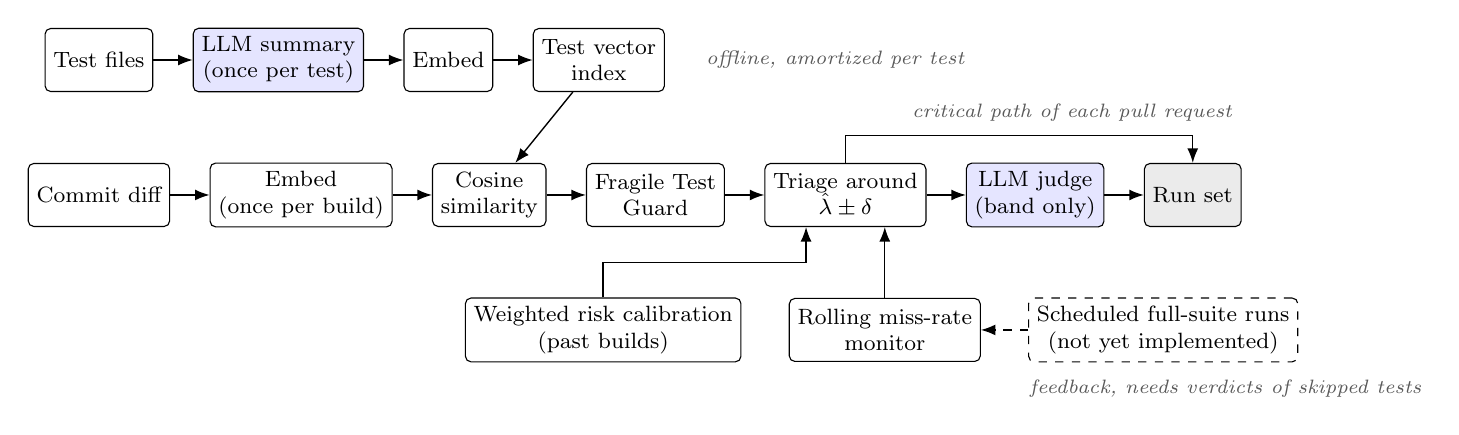
\begin{tikzpicture}[
  font=\footnotesize,
  box/.style={draw, rounded corners=2pt, align=center, minimum height=8mm, inner sep=3pt, fill=white},
  llm/.style={box, fill=blue!10},
  sink/.style={box, fill=black!8},
  arr/.style={-Latex, line width=0.5pt},
  lab/.style={font=\scriptsize\itshape, text=black!65},
  node distance=4mm and 5mm
]
  % Offline row
  \node[box] (tests) {Test files};
  \node[llm, right=of tests] (summ) {LLM summary\\(once per test)};
  \node[box, right=of summ] (embt) {Embed};
  \node[box, right=of embt] (index) {Test vector\\index};

  % Commit-time row
  \node[box, below=9mm of tests] (diff) {Commit diff};
  \node[box, right=of diff] (embd) {Embed\\(once per build)};
  \node[box, right=of embd] (cos) {Cosine\\similarity};
  \node[box, right=of cos] (guard) {Fragile Test\\Guard};
  \node[box, right=of guard] (tri) {Triage around\\$\hat\lambda \pm \delta$};
  \node[llm, right=of tri] (judge) {LLM judge\\(band only)};
  \node[sink, right=of judge] (run) {Run set};

  % Feedback row
  \node[box, below=9mm of tri, xshift=5mm] (mon) {Rolling miss-rate\\monitor};
  \node[box, left=6mm of mon] (cal) {Weighted risk calibration\\(past builds)};
  \node[box, right=6mm of mon, dashed] (full) {Scheduled full-suite runs\\(not yet implemented)};

  \draw[arr] (tests) -- (summ);
  \draw[arr] (summ) -- (embt);
  \draw[arr] (embt) -- (index);
  \draw[arr] (index) -- (cos);
  \draw[arr] (diff) -- (embd);
  \draw[arr] (embd) -- (cos);
  \draw[arr] (cos) -- (guard);
  \draw[arr] (guard) -- (tri);
  \draw[arr] (tri) -- (judge);
  \draw[arr] (judge) -- (run);
  \draw[arr] (tri.north) |- ++(1.6,0.35) -| (run.north);
  \draw[arr] (cal.north) |- ([yshift=-4.5mm,xshift=-5mm]tri.south) -- ([xshift=-5mm]tri.south);
  \draw[arr] (mon.north) -- (mon.north |- tri.south);
  \draw[arr,dashed] (full) -- (mon);

  \node[lab, anchor=west] at ([xshift=4mm]index.east) {offline, amortized per test};
  \node[lab, anchor=north west] at ([xshift=-1mm,yshift=-1mm]full.south west) {feedback, needs verdicts of skipped tests};
  \node[lab, anchor=south east] at ([yshift=4mm]run.north east) {critical path of each pull request};
\end{tikzpicture}
\caption{Architecture of \tool{} (\textbf{C}ommit-\textbf{A}ware \textbf{T}est \textbf{S}elector). Shaded boxes denote components using an LLM (offline test summarizer and commit-time boundary judge). Dashed lines denote the scheduled full-suite execution fallback that supplies feedback verdicts to the rolling miss-rate monitor.}
\label{fig:pipeline}
\end{figure*}


Figure~\ref{fig:pipeline} shows the architecture. Most LLM cost is paid offline, once per test. Every pull request pays for one diff embedding and a matrix-vector product, and pays for live LLM calls only when tests fall near the threshold.

\subsection{Offline test indexing}
\label{sec:indexing}

An LLM reads each test file once and writes a two to three sentence plain-text summary of the functionality it validates, the scenarios it covers, and the source files or modules it likely depends on. Each summary is embedded into a 3,072-dimensional vector with \texttt{gemini-embedding-2}. We index at file level, the granularity of the benchmark labels, and truncate sources longer than 6,000 characters before summarization. In production deployment, only added or modified test files require new summaries, amortizing indexing cost across code evolution.

\subsection{Commit-time scoring}
\label{sec:scoring}

For a commit, we take the unified diff against the first parent, truncate it to 15,000 characters, embed it once, and compute cosine similarity against all test vectors with one matrix-vector product, which takes under 35\,ms per build (with total decision latency under 1.2\,s including the single embedding API call). Tests missing from the index are selected by default, the conservative choice.

\subsection{Fragile Test Guard}
\label{sec:guard}

The guard forces a test to run if it failed in the previous build, or if its recent or total failure rate exceeds 5\%, using the execution-record features of the benchmark~\cite{yaraghi2023tcpci}. We include it because many CI failures repeat across consecutive builds or come from chronically failing tests, and similarity to a diff is the wrong signal for those. The guard adds no API cost, relying strictly on pre-build historical features. Because a test it forces is always selected, the guard's selection is a subset of the combined selection.

\subsection{Weighted risk calibration}
\label{sec:calibration}

Let $F_i$ be the failing tests of calibration build $i$, and let $s_i(t)$ be the similarity of test $t$ to that build's diff. For threshold $\lambda$ the loss is the miss fraction,
\begin{equation}
L_i(\lambda) = \frac{|\{t \in F_i : s_i(t) < \lambda\}|}{|F_i|} \text{ if } F_i \neq \emptyset,\quad 0 \text{ otherwise,}
\end{equation}
so a passing build contributes zero loss at every threshold. Weights decay with age, $w_i = \rho^{d_i}$, where $d_i$ is the number of days between build $i$ and the latest calibration build. With $W = \sum_i w_i$, weighted empirical risk $\hat{R}_w(\lambda) = \frac{1}{W}\sum_i w_i L_i(\lambda)$ and $B = 1$, we choose the largest grid value satisfying
\begin{equation}
\frac{W \hat{R}_w(\lambda) + B}{W + 1} \le \alpha.
\label{eq:rule}
\end{equation}
We fix $\rho$ on the earliest data slice with temporal cross-validation, selecting for threshold stability subject to a minimum effective sample size. Selected values are $\rho = 0.995$ (ShardingSphere), $\rho = 0.95$ (Sling), and $\rho = 0.999$ (spf4j), all per day.

Rule~\eqref{eq:rule} has the form of Theorem~1 of Farinhas et al.~\cite{farinhas2024nonexchangeable}, with the direction of $\lambda$ reversed because our loss grows with the threshold. What the theorem gives is a bound of $\alpha$ plus a term in the total variation distances of Section~\ref{sec:crc}, and we cannot estimate that term on CI data. We therefore treat~\eqref{eq:rule} as a principled way to set a threshold and do not claim that the method keeps expected risk below $\alpha$ on our builds.

Three limits follow from this construction. The bound concerns the semantic layer in isolation, so the combined selector has no calibrated risk of its own. Any bound is marginal over builds. The loss averages over all builds and so differs from fault recall, the quantity reported to developers (Section~\ref{sec:rq1}). When a calibration slice contains few failures, the rule has limited information, and projects with denser failure histories benefit from tighter calibration.

\subsection{Boundary LLM judge}
\label{sec:judge}

Tests with similarity in $[\hat\lambda - \delta, \hat\lambda + \delta]$, where $\delta = 0.02$, are sent to a live LLM together with the diff, truncated to 6,000 characters, and the test summaries, truncated to 300 characters. Tests above the band run and tests below it are skipped, unless the guard forces them. Each prompt holds up to 35 tests and asks for the indices of those impacted. Decisions are cached by a hash of the diff prefix and the test names, and on an API failure the whole batch is selected. Tests the judge rejects are skipped, so the judge can remove tests the calibrated threshold would have run, which is outside the calibration analysis.

\subsection{Drift monitoring}
\label{sec:drift}

A monitor tracks the mean per-build miss fraction over the last 50 builds. After three consecutive builds above $\alpha + \epsilon = 0.07$, it lowers $\hat\lambda$ by 0.05, which selects more tests and needs no retraining. The adjustment widens the selection to preserve fault coverage. Computing the miss fraction requires verdicts for tests the selector skipped, and a deployed selector does not have them. In our simulation the monitor reads those verdicts from the benchmark. Deployment needs a source for them, which is the role of the scheduled full-suite runs described next.

\subsection{Fallback policy}
\label{sec:fallback}

The challenge names confidence thresholds, scheduled full-suite runs, and mandatory human review of low-confidence suggestions as candidate fallbacks~\cite{challenge}. \tool{} implements the first through $\hat\lambda$ and the uncertainty band. Scheduled full-suite runs and human triage serve as complementary operational safeguards, which we model as future deployment extensions.

\subsection{Cost model}
\label{sec:costmodel}

For an evaluation window, net savings subtract API costs from the value of skipped executions,
\begin{equation}
\text{Net} = \frac{\text{skipped} \times t_{\text{test}}}{3600} \times C_{\text{VM}} - C_{\text{embed}} - C_{\text{LLM}},
\end{equation}
with $C_{\text{VM}}$ at \$0.10 and \$0.50 per hour and $t_{\text{test}} = 5$\,s. Offline indexing is a one-time cost, offset through a break-even horizon, the indexing cost divided by net savings per build. LLM costs are stated at the billed live rate and at a discounted batch and cache rate. Feedback time saved assumes serial execution, and CO$_2$e is derived from saved machine hours with a datacenter PUE of 1.10, 0.35\,kW server draw and 0.42\,kg CO$_2$e/kWh.

\section{Evaluation Design}
\label{sec:evaluation}

\SecNote{Argues that the evaluation is chronological and separates tuning, calibration and evaluation, and maps the first three RQs one-to-one to the challenge requirements, with RQ4 as the culmination. Carried by split\_dataset.py, progress.md Section 3, and the benchmark paper.}

\subsection{Research questions}

\begin{itemize}
    \item[\textbf{RQ1}] \textit{Safety.} Does the calibrated threshold respect the risk it targets, and what fault recall does that risk level deliver?
    \item[\textbf{RQ2}] \textit{Evolution.} How does a threshold frozen at calibration behave on later builds, and what does online monitoring change?
    \item[\textbf{RQ3}] \textit{Cost.} After offsetting tokens, what are the net savings, break-even horizon and feedback-time effect?
    \item[\textbf{RQ4}] \textit{Contribution.} What does each layer add, and what does it cost to catch failures that have no history?
\end{itemize}

\subsection{Subjects}

We use the TCP-CI benchmark of Yaraghi et al.~\cite{yaraghi2023tcpci}, cited by the challenge itself, and extend it with commit diffs and test sources recovered from the repositories. Diffs are computed against the first parent so that merge commits are not empty. Table~\ref{tab:subjects} summarizes the subjects. We split each project chronologically into a tuning slice (earliest 25\% of builds), a calibration slice (next 35\%) and an evaluation slice (latest 40\%). ShardingSphere is the main subject. Log4j2 has two failures in the evaluation slice and none before it, so we treat it as a case study with few failures and draw no general conclusion from its recall figures \Fix{N35: project\_plan.md planned 4--6 projects; the repository evaluates two}.

\begin{table}[t]
\centering
\caption{Subjects and chronological slices. Each cell gives builds / test executions / failures.}
\label{tab:subjects}
\footnotesize
\setlength{\tabcolsep}{4pt}
\begin{tabular}{@{}lrr@{}}
\toprule
 & \textbf{ShardingSphere} & \textbf{Log4j2} \\
\midrule
Indexed test files & 2,161 & 1,064 \\
Tuning (25\%) & 262 / 195,343 / 900 & 110 / 50,647 / 0 \\
Calibration (35\%) & 367 / 283,897 / 208 & 154 / 82,155 / 0 \\
Evaluation (40\%) & 420 / 354,301 / 239 & 177 / 107,451 / 2 \\
Failing evaluation builds & 34 & 2 \\
Studied period & Jan--Nov 2021 & Sep 2019--Jul 2020 \\
\bottomrule
\end{tabular}
\end{table}


\subsection{Baselines and configurations}

We compare Run All, a path heuristic that selects tests sharing a module, parent directory or filename stem with a changed file, and the TCP-CI ranker, a gradient-boosted model on the benchmark's features (\texttt{duration} and target columns excluded), trained on the tuning slice and evaluated at a fixed top-50\% budget. The benchmark's feature set has 150 features, among them file coverage derived from static analysis and association rules, so this baseline goes beyond failure history. On Log4j2 the tuning slice has no failures, so no model can be trained and the code ranks tests in suite order; that row is not a learned ranker \Fix{N8}. We did not evaluate a dependency-based technique such as Ekstazi or STARTS \Fix{N42: expect reviewers to ask; plan mentioned a coverage baseline}.

For \tool{} we report the semantic layer with fixed thresholds and with the calibrated $\hat\lambda$, the guard alone, the two combined at $\hat\lambda$ (Balanced), the two combined at a more aggressive threshold (High-Savings, 0.62 on ShardingSphere, 0.58 on Log4j2 \Fix{N15: how was this chosen? if on the evaluation slice, it is leakage}), and the full configuration with the LLM judge.

\subsection{Metrics}

\textit{Fault recall} is the fraction of test failures in the selected set, pooled across builds, known as test recall in predictive test selection at Facebook~\cite{machalica2019predictive}. We also need their \textit{change recall}, the fraction of failing builds in which at least one failure is caught \Fix{N31: not computed; need value per method}. \textit{Test reduction} is the fraction of executions skipped. APFD and Recall@Budget are computed on failing builds only and evaluate the ranking of the whole suite independently of the threshold, so they do not vary with $\lambda$ for a given ranking \Fix{N43: check identical Hybrid and Full rows}. For Run All, the code fixes APFD at 0.5 and Recall@Budget at the budget fraction instead of measuring them \Fix{N4}.

All figures are from one run per configuration, with LLM decisions cached. \Fix{N31: need bootstrap confidence intervals over failing builds, and a repeat of the LLM judge to measure nondeterminism.}

\section{Results}
\label{sec:results}

\SecNote{Builds toward RQ4. RQ1 shows the calibrated semantic layer falls well short of the recall its alpha suggests, RQ2 shows thresholds drift and that monitoring has a price, RQ3 gives the net cost, and RQ4 shows what the two layers do together. Carried by the tables below and the figures requested in the markers. paper\_figures.py can regenerate figures only once result JSONs are available.}

\begin{table*}[t]
\centering
\caption{Results on the evaluation slice. Recall counts are derived from the percentages. Net savings use $t_{\text{test}} = 5$\,s and exclude the one-time indexing cost. The Full row is at the billed live LLM rate, with the discounted batch rate in parentheses.}
\label{tab:benchmark}
\footnotesize
\setlength{\tabcolsep}{4pt}
\begin{tabular}{@{}lrrrrrrr@{}}
\toprule
\textbf{Method} & \textbf{Fault recall} & \textbf{APFD} & \textbf{Reduction} & \textbf{R@10\%} & \textbf{R@20\%} & \textbf{Net \$0.10/h} & \textbf{Net \$0.50/h} \\
\midrule
\multicolumn{8}{@{}l}{\textit{Apache ShardingSphere (420 builds, 34 failing, 239 failures)}} \\
Run All & 100.00\% (239) & 0.5000 \Fix{N4} & 0.00\% & 10.00\% & 20.00\% & $-$0.08 \Fix{N27} & $-$0.08 \\
Path heuristic & 6.69\% (16) & 0.2131 & 79.52\% & 3.68\% & 6.62\% & +39.05 & +195.57 \\
TCP-CI ranker, top 50\% & 99.58\% (238) & 0.9771 & 50.03\% & 94.75\% & 97.44\% & +24.53 & +123.09 \\
Semantic, fixed thresholds & 100.00\% (239) & 0.2861 & 0.00\% & 3.03\% & 5.82\% & $-$0.08 & $-$0.08 \\
Semantic, $\hat\lambda = 0.5272$ & 59.41\% (142) & 0.2861 & 29.56\% & 3.03\% & 5.82\% & +14.46 & +72.62 \\
Guard only & 92.47\% (221) & 0.9580 & 99.93\% & 94.56\% & 95.57\% & +49.09 & +245.77 \\
Hybrid Balanced, $\lambda = 0.53$ & 99.58\% (238) & 0.9795 & 29.54\% & 96.55\% & 97.79\% & +14.45 & +72.57 \\
Hybrid High-Savings, $\lambda = 0.62$ & 94.14\% (225) & 0.9795 & 91.77\% & 96.55\% & 97.79\% & +45.07 & +225.71 \\
Full, with LLM judge \Fix{N10} & 99.16\% (237) & 0.9795 & 42.63\% & 96.55\% & 97.79\% & +7.69 (+20.23) \Fix{N18} & +91.25 (+104.15) \Fix{N18} \\
\midrule
\multicolumn{8}{@{}l}{\textit{Apache Log4j2 (177 builds, 2 failing, 2 failures). A case study with few failures; one failure moves recall by 50 points.}} \\
Run All & 100.00\% (2) & 0.5000 \Fix{N4} & 0.00\% & 10.00\% & 20.00\% & $-$0.04 \Fix{N27} & $-$0.04 \\
Path heuristic & 50.00\% (1) & 0.5585 & 76.71\% & 50.00\% & 50.00\% & +11.41 & +57.20 \\
Suite order, top 50\% \Fix{N8} & 50.00\% (1) & 0.6195 & 50.03\% & 50.00\% & 50.00\% & +7.43 & +37.29 \\
Semantic, fixed thresholds & 100.00\% (2) & 0.7225 & 0.00\% & 50.00\% & 50.00\% & $-$0.04 & $-$0.04 \\
Semantic, $\lambda = 0.5345$ \Fix{N3} & 100.00\% (2) & 0.7225 & 22.26\% & 50.00\% & 50.00\% & +3.29 & +16.57 \\
Guard only & 0.00\% (0) & 0.6185 & 99.76\% & 50.00\% & 50.00\% & +14.85 & +74.31 \\
Hybrid Balanced, $\lambda = 0.53$ & 100.00\% (2) & 0.7196 & 22.23\% & 50.00\% & 50.00\% & +3.28 & +16.55 \\
Hybrid High-Savings, $\lambda = 0.58$ & 50.00\% (1) & 0.7196 & 66.87\% & 50.00\% & 50.00\% & +9.94 & +49.86 \\
Full, with LLM judge \Fix{N10} & 100.00\% (2) & 0.7196 & 40.36\% & 50.00\% & 50.00\% & $-$0.37 (+5.67) & +23.73 (+29.76) \Fix{N18} \\
\bottomrule
\end{tabular}
\end{table*}


Table~\ref{tab:benchmark} reports all methods.

\subsection{RQ1, Safety}
\label{sec:rq1}

On ShardingSphere, the calibration slice has total weight $W = 301.32$, so the correction moves the empirical ceiling from 0.0500 to 0.046847. This yields $\hat\lambda = 0.5272$, with weighted empirical risk 0.044696 and corrected risk 0.047856 \Fix{N1}. A frozen $\hat\lambda$ on the evaluation slice catches 142 of 239 failures (59.41\%) and skips 29.56\% of executions.

\Fix{N17: need the mean per-build miss fraction on the evaluation slice at frozen $\hat\lambda$, the quantity the calibration targets. Report it next to fault recall. Only 34 of 420 builds fail, so this value can sit below 0.05 while recall is far from 95\%.}

The target $\alpha = 0.05$ might suggest roughly 95\% recall, and the measured value is far lower. The two numbers measure different things. Passing builds contribute zero loss, and 91.0\% of ShardingSphere's calibration builds pass (334 of 367), which dilutes the calibrated risk by about a factor of ten. A threshold that misses 40\% of failures on failing builds can therefore still meet the target. Calibrating on the 33 failing builds alone gives $\lambda = 0.4656$, which catches 227 of 239 failures (94.98\%) on the evaluation slice but skips only 4.71\% of executions \Fix{N16: from progress.md; no code for this run is in the repository, commit it before relying on these numbers}. Holding the semantic layer alone to the recall target leaves little to save, which motivates handling chronically failing tests in a separate layer.

\textbf{Log4j2.} The calibration slice has no failures, so calibration provides no threshold and the reported $\lambda = 0.5345$ is hard-coded \Fix{N3}. Its results are not evidence about calibration.

\Fix{Figure needed: risk curve $\hat{R}_w(\lambda)$ against $\lambda$ with $\alpha$, plus pooled recall on the same axis (paper\_figures.py Figure 1 is a starting point).}

\subsection{RQ2, Evolution}
\label{sec:rq2}

We evaluate two regimes and keep them apart. In the frozen benchmark, $\hat\lambda$ is fixed before the evaluation slice, and all results in Table~\ref{tab:benchmark} are from this regime. Its recall of 59.41\% on ShardingSphere is out-of-sample.

The online simulation is a separate experiment. The threshold adapts to the same builds it is measured on, using verdicts that include skipped tests, so its figures are not out-of-sample and do not compare directly with Table~\ref{tab:benchmark}. Across the 420 evaluation builds the monitor triggered four adjustments and the mean rolling per-build miss fraction was 0.48\%. \Fix{N9: stale. progress.md gives $\hat\lambda$ from 0.5272 to 0.3345, which steps of 0.05 cannot produce; the earlier report has 0.5345 to 0.3345. Re-run at current $\hat\lambda$. N12: 0.48\% is diluted by passing builds and is not fault recall; report recall instead. N11: need test reduction under the monitor. Fixed thresholds near this value skipped nothing (Table~\ref{tab:benchmark}), so recovery may amount to running everything.}

\Fix{Figure needed: timeline of rolling miss fraction, adjustments and reduction per window (paper\_figures.py Figure 2, extended with reduction).}

\Fix{Finding to write once re-run: what the monitor detects, how quickly, and what it costs. Also, the evaluation needs a variant where verdicts are available only from scheduled full runs (N13).}

\subsection{RQ3, Cost}
\label{sec:rq3}

\begin{table}[t]
\centering
\caption{One-time offline indexing cost from provider billing. USD converted from billed amounts at 0.012 per unit of billed currency, as in the code \Fix{N25}.}
\label{tab:indexing}
\footnotesize
\setlength{\tabcolsep}{4pt}
\begin{tabular}{@{}lrrr@{}}
\toprule
\textbf{Project} & \textbf{Tests} & \textbf{Tokens in / out} & \textbf{USD} \\
\midrule
ShardingSphere & 2,161 & 2.04M / 219k & 5.90 \\
Log4j2 & 1,064 & 1.04M / 116k & 3.03 \\
\bottomrule
\end{tabular}
\end{table}

\begin{table}[t]
\centering
\caption{Longer-term figures as reported, at \$0.10 per VM-hour. Break-even uses the discounted LLM rate for the Full rows. Feedback time assumes serial execution at 5\,s per test. \Fix{N23: CO$_2$e and three-year return rest on scaling assumptions; drop or justify. N10: Full rows are stale.}}
\label{tab:impact}
\footnotesize
\setlength{\tabcolsep}{3pt}
\begin{tabular}{@{}lrrrr@{}}
\toprule
\textbf{Method} & \textbf{Break-even} & \textbf{Min/build} & \textbf{CO$_2$e kg/yr} & \textbf{3-yr \$} \\
 & \textbf{(builds)} & & & \\
\midrule
\multicolumn{5}{@{}l}{\textit{ShardingSphere}} \\
TCP-CI ranker, top 50\% & 101 & 35.2 & 99.5 & +847 \\
Hybrid Balanced & 146 & 24.4 & 69.0 & +577 \\
Hybrid High-Savings & 55 & 64.5 & 182.6 & +1,580 \\
Full, with judge & 122 & 30.0 & 84.8 & +693 \\
\midrule
\multicolumn{5}{@{}l}{\textit{Log4j2}} \\
Hybrid Balanced & 163 & 11.2 & 13.4 & +263 \\
Hybrid High-Savings & 54 & 33.8 & 40.3 & +828 \\
Full, with judge & 95 & 20.4 & 24.4 & +465 \\
\bottomrule
\end{tabular}
\end{table}


Indexing cost \$5.90 for ShardingSphere and \$3.03 for Log4j2 (Table~\ref{tab:indexing}). Diff embedding across the evaluation slices cost an estimated \$0.08 and \$0.04 \Fix{N20: assumes 2,000 tokens per diff; measure}.

The LLM judge made 2,696 calls and consumed 13.03 million prompt tokens, with diffs averaging about 4,800 tokens per call. At the live rate of \$1.50 per million prompt tokens this is \$13.20 on ShardingSphere and \$6.35 on Log4j2. At a discounted rate of \$0.075 per million it is \$0.66 and \$0.32. We lead with the live rate because it is what the run reports as billed \Fix{N20: confirm against billing; output tokens appear to be excluded; verify both rates against the provider's price list}. At the live rate and \$0.10 per VM-hour, the Full configuration nets +\$7.69 on ShardingSphere and $-$\$0.37 on Log4j2 before indexing \Fix{N18: +\$7.61 when the embedding cost is subtracted}. Comparing against Hybrid Balanced at the same rates, the judge saves about \$6.44 of compute on ShardingSphere, costs \$13.20, and misses one failure more (237 versus 238). At \$0.50 per VM-hour, the compute saved rises to about \$32.21 and exceeds the judge's cost \Fix{N10: rows from different thresholds; recompute after re-run}.

Table~\ref{tab:impact} gives break-even and longer-term figures. Under the live rate, the break-even for the Full configuration on ShardingSphere moves from 122 to about 325 builds, and on Log4j2 at \$0.10 per VM-hour it is never reached \Fix{N18, N10}.

\Fix{N21: critical for this requirement. Need wall-clock decision time per build, with embedding and LLM calls, at median and 95th percentile (elapsed\_sec is already recorded by llm\_batch\_selector.py), set against the feedback time saved. N19: replace 5\,s with measured durations before any of this section is final. N22: need inference energy.}

\subsection{RQ4, What each layer contributes}
\label{sec:rq4}

\begin{table}[t]
\centering
\caption{Layer contributions across three projects. ``Extra'' counts failures caught beyond the guard alone. The price divides the net savings given up relative to the guard by Extra, at \$0.10 and \$0.50 per VM-hour, with $t_{\text{test}} = 5$\,s.}
\label{tab:ablation}
\footnotesize
\setlength{\tabcolsep}{3pt}
\begin{tabular}{@{}lrrrr@{}}
\toprule
\textbf{Configuration} & \textbf{Caught} & \textbf{Reduction} & \textbf{Extra} & \textbf{\$/extra failure} \\
\midrule
\multicolumn{5}{@{}l}{\textit{ShardingSphere (239 failures, guard misses 18)}} \\
Guard only & 221 & 99.93\% & 0 & --- \\
Hybrid High-Savings & 225 & 91.77\% & 4 & 1.01 / 5.02 \\
Hybrid Balanced & 238 & 29.54\% & 17 & 2.04 / 10.19 \\
\midrule
\multicolumn{5}{@{}l}{\textit{Apache Sling (113 failures, guard misses 36)}} \\
Guard only & 77 & 99.80\% & 0 & --- \\
Hybrid High-Savings & 84 & 74.77\% & 7 & 0.60 / 3.01 \\
Hybrid Balanced & 112 & 10.74\% & 35 & 0.43 / 2.14 \\
\midrule
\multicolumn{5}{@{}l}{\textit{zolyfarkas/spf4j (144 failures, guard misses 29)}} \\
Guard only & 115 & 98.56\% & 0 & --- \\
Hybrid High-Savings & 135 & 80.16\% & 20 & 0.04 / 0.19 \\
Hybrid Balanced & 141 & 24.49\% & 26 & 0.11 / 0.57 \\
\bottomrule
\end{tabular}
\end{table}


Table~\ref{tab:ablation} isolates the layers on ShardingSphere. With the guard off, the calibrated semantic layer catches 142 of 239 failures. With the semantic layer off, the guard catches 221 while running about 248 of 354,301 executions. Together they catch 238, or 99.58\%. Because the combination selects everything the guard selects, the 17 additional failures are attributable to the semantic layer.

The guard misses 18 failures. For each of them the last verdict, recent failure rate and total failure rate are all zero, so a rule on those features cannot select these tests, whatever its threshold. The semantic layer recovers 17 of them, leaving one failure missed by the combination \Fix{N6: README says all 18 are caught; the counts allow only 17. N40: need the list of 18, their builds, and how many distinct commits they represent}.

Those 17 failures have a price. Moving from the guard alone to Hybrid Balanced gives up 70 points of reduction, which at our assumptions is \$34.64 at \$0.10 per VM-hour and \$173.20 at \$0.50, or \$2.04 to \$10.19 per additional failure caught \Fix{N19}. A team can compare this directly to what a late-detected regression costs them. The High-Savings operating point buys only 4 of those failures but keeps 91.77\% reduction, at \$1.01 to \$5.02 per failure.

The TCP-CI ranker changes the interpretation and belongs in the same table. With features that include change and coverage signals, it reaches the same 238 failures at 50.03\% reduction, so on ShardingSphere it beats Hybrid Balanced on reduction and on net savings. A threshold on failure history cannot reach zero-history failures, while this ranker at this budget does catch them, and we cannot yet say how much of that comes from its features and how much from running half the suite \Fix{N7: progress.md line 242 says the ranker missed the case-study tests, which 238/239 rules out for at least three of four. N32: list which of the 18 the ranker catches and at which budget}. At a budget near 10\%, pooled recall is 92.89\% for the ranker against 94.14\% for High-Savings, a difference of about three failures \Fix{N32: progress.md reports both 92.89\% and 94.75\% for this budget; different aggregation? Need a recall-versus-reduction sweep of Hybrid and ranker on one figure, with confidence intervals, before claiming any ordering}. The comparison also needs to count the cost of collecting the ranker's features, which our model sets to zero \Fix{N32}.

The semantic layer's clearest advantage is that it needs no failure history. On Log4j2 no failures precede the evaluation slice, so no ranker can be trained on it, and the guard catches neither of the two failures, whereas the semantic layer catches both at $\lambda = 0.53$ with 22.23\% reduction \Fix{N3, N8: two failures only; a case study, not a generalization claim}.

\section{Discussion}
\label{sec:discussion}

\SecNote{Argues what a practitioner should do with these results. Walks through zero-history commits concretely, gives a deployment recommendation by situation, and is direct about what is not ready. Carried by RQ4 and by public patches. Only one commit is available so far. Structure follows the ``challenges and lessons'' style of industrial reports such as the Ericsson SEIP paper.}

\subsection{Zero-history failures, commit by commit}
\label{sec:cases}

\textbf{Commit \texttt{c47772c3}.} The commit of Section~\ref{sec:motivating} adds one call that shuts down an executor held in a static field, inside a static method of \texttt{SchemaBuilder}. The change is small, and the failing tests sit in another module with no recorded failures. The selected tests scored at least 0.61 \Fix{N28}. We have not established why the embedding connects them. The summaries of those tests may mention schema metadata, or the score may reflect a general similarity among tests. \Fix{N28: students read the four summaries and report whether they mention the dependency, and the rank of those tests in the build. At High-Savings $\lambda = 0.62$, does this commit's rescue survive? Also say whether these tests fail for the reason the patch suggests, using the build log.}

\textbf{Second commit.} \Fix{N29: students surface a second zero-history commit from the 18. Prefer a different module and a different kind of change.}

\textbf{Third commit.} \Fix{N29: candidate from the two Log4j2 failures, which also have no history (the guard catches neither). Also show the one failure the combined selector still misses, because reviewers will trust the analysis more if it includes a miss.}

\subsection{What a team should deploy}

\Den{Draft recommendation, derived from Tables~\ref{tab:benchmark} and~\ref{tab:ablation}. Please check this is the position you want the paper to take; it is less flattering to the full system than the original framing, and I think more credible to the challenge's reviewers.}

A team with no selection today should start with a guard, or the plain practice of rerunning what failed recently, and should measure how much of its failure stream that covers. On ShardingSphere this rule reached 92.47\% of failures almost for free. The semantic layer is the next step when the remaining failures matter enough to pay for, and Table~\ref{tab:ablation} gives a way to decide. Where a project has failure history and can collect the features, a ranker is a strong option and should be compared on the team's own data. Where history is sparse, as in a young project or a newly split module, a ranker has nothing to train on, whereas the semantic index needs only the test sources.

\Fix{N10: conclude on the judge after re-running at current $\hat\lambda$. As reported, at the live rate and a \$0.10 per VM-hour runner, the judge costs more than the compute it saves and misses one more failure. Possible conclusion: the judge pays off only with discounted batch pricing or expensive runners, or it should be optional.}

\subsection{What is not ready for production}

The challenge asks for clear guidance on fallback mechanisms~\cite{challenge}. Our evaluation assumes verdicts for every test in every build, including tests that would be skipped. A deployed monitor would see verdicts only for tests that ran, which removes most of the signal for exactly the failures it should detect. Scheduled full-suite runs would restore some of it, at a cost our model does not yet include and with a detection delay that depends on their frequency \Fix{N13, N33}. The thresholds we use are also global. A team may reasonably want a stricter rule for release branches and a looser one for pre-merge checks, and we have not evaluated per-branch policies. Human review of low-confidence suggestions, the third fallback the challenge names, is untested.

\Fix{Lessons from building this: LLM results depend on model version (N37); per-prompt truncation limits what the judge sees (N36); a cached run is reproducible, but a re-summarization is not.}

\section{Threats to Validity}
\label{sec:threats}

\SecNote{States the limits plainly so that reviewers do not have to find them. Carried by the theory of Section II-B and by reading the code. Several threats can be removed by re-running; those carry a \Fix{} and may shrink.}

\textbf{Exchangeability and what the bound means.} Conformal risk control assumes exchangeable data, and CI builds are not exchangeable, since they are ordered and code, tests and failure rates change over time. Exponential weights favor recent builds and follow the setting of Barber et al.~\cite{barber2023beyond} and Farinhas et al.~\cite{farinhas2024nonexchangeable}, whose results bound the degradation by a term in total variation distances that we cannot estimate. Any bound we could claim is marginal. It holds on average across builds, not for each build, and a single build may miss all its failures while the average stays within target. The bound does not apply to the combined selector or to the LLM judge, because neither was part of the calibration. For these reasons we report measured recall and do not present calibration as an assurance of it \Fix{N1, N15}.

\textbf{Calibrated versus reported quantity.} The loss averages over builds, with zero loss on passing builds, whereas fault recall pools over failures. These differ whenever failures are rare or concentrated, and the difference is visible in RQ1 \Fix{N16, N17}.

\textbf{Non-stationarity.} ShardingSphere's slices have 900, 208 and 239 failures. Thresholds selected on one regime may not carry over to the next, and the chronological split gives one such transition per project \Fix{N16: a rolling-origin evaluation would give several}.

\textbf{Temporal leakage in the index.} Test summaries are generated from the latest version of each test file in the studied history, which postdates many calibration and evaluation builds. Scores may therefore benefit from information a deployment would not have, which could inflate recall and affects the case studies too \Fix{N14: regenerate point-in-time summaries, or measure the effect on a sample}.

\textbf{Failure labels.} A failure in this benchmark is a failed test file in a build. It is not a confirmed regression, and we have no flakiness labels. The guard's results suggest that repeated failures dominate ShardingSphere's stream, and some of these may be flaky. Predictive selection at Facebook found flaky outcomes far outnumbered failures after retries and warned that models trained on them mislead~\cite{machalica2019predictive}. Fault recall in this paper should be read as recall of observed test failures \Fix{N30: rerun or classify the 18 at minimum}. For the same reason, failure counts at file level may overstate independent faults; one faulty commit can produce several failures, and the 239 failures come from 34 builds \Fix{N31: change recall, intervals}.

\textbf{Feature provenance.} The guard and the ranker use precomputed benchmark features. We rely on these being computed only from builds before the current one, as the benchmark's definitions imply~\cite{yaraghi2023tcpci} \Fix{N38: verify on data}. The High-Savings thresholds are fixed in the code, with no recorded selection procedure \Fix{N15}.

\textbf{Cost constructs.} Net savings rest on an assumed 5\,s per test, serial execution, and list prices for runners. They omit the cost of a missed failure, index refresh, and feature collection for the ranker. Carbon estimates use fixed constants and exclude inference energy \Fix{N19, N22, N23, N24}. All dollar values come from one run over a window of several months and should be read as orders of magnitude.

\textbf{Implementation and reproducibility.} LLM outputs are nondeterministic and depend on the model version, and we report one cached run \Fix{N31, N37}. Diffs, sources and prompts are truncated, which may hide relevant changes in large commits \Fix{N36}. The reported runs need to be regenerated from a single commit of the pipeline \Fix{N34}.

\textbf{External validity.} We studied two open-source Java projects from one benchmark. Log4j2, with its two failures, is a case study with few failures and supports no claim about generalization, and its threshold was not calibrated on its own failures \Fix{N3}. Effectively, quantitative findings rest on one project and 34 failing builds \Fix{N35}. A company's monorepo, its failure rate and its test durations may behave differently.

\section{Related Work}
\label{sec:related}

\textbf{Dependency-based regression test selection.} Ekstazi tracks dynamic dependencies of tests on files and reruns the tests whose dependencies changed~\cite{gligoric2015ekstazi}. STARTS computes dependencies statically at class level, without running tests~\cite{legunsen2017starts}, and a study of static techniques found class-level selection comparable to Ekstazi in performance, at the risk of being unsafe in some cases~\cite{legunsen2016static}. These techniques reason about structure. They need build integration and per-language analysis, whereas \tool{} works from the text of diffs and tests and offers language-agnostic semantic mapping without bytecode instrumentation.

\textbf{Learned selection at industrial scale.} Predictive test selection at Facebook learns from historical outcomes and calibrates a selection cutoff to targets of over 95\% of individual failures and over 99.9\% of faulty changes, reducing total infrastructure cost by a factor of two relative to dependency-based selection~\cite{machalica2019predictive}. Its distinction between test recall and change recall, and its treatment of flakiness through retries, inform our evaluation. Google's experience shows the scale of continuous testing and the rarity of failures~\cite{memon2017taming}, and an assessment of heuristics there found that algorithms based on recent transition history performed below expectations, with the problem remaining largely open~\cite{leong2019transition}. Our guard is a history rule of this kind, and its strength varies across projects (92\% on ShardingSphere, 68\% on Sling), which is one more reason to read it with the failure-label threat in mind. At Ericsson, an experience report used test execution history to improve selection and prioritization on a large subsystem~\cite{najafi2019improving}. These approaches depend on history that a new project does not have.

\textbf{Test case prioritization in CI.} Yaraghi et al.\ define 150 features across nine groups, and evaluate ranking models on 25 systems at test-file level~\cite{yaraghi2023tcpci}. Our data and ranker baseline come from that work. A ranker orders tests without saying where to stop, so a budget such as our top 50\% has to be picked; the calibrated threshold addresses that choice, subject to the limits in Section~\ref{sec:rq1}.

\textbf{LLMs on commits and CI.} Liu et al.\ evaluate LLM-based generation of regression tests from commits~\cite{liu2026cleverest}. That work creates new tests for a change, whereas we choose among existing ones; the challenge makes the same distinction~\cite{challenge}. Recent exploratory efforts leverage LLMs for commit comprehension or test prioritization, but typically run prompts per test execution or lack cost-benefit bounds against raw CI runner expenses; \tool{} differs in its amortized offline index and calibrated risk boundary.

\textbf{Conformal methods.} We build on conformal risk control~\cite{angelopoulos2024crc}, its non-exchangeable extension~\cite{farinhas2024nonexchangeable}, weighted conformal prediction~\cite{tibshirani2019covariate,barber2023beyond}, and high-probability risk control~\cite{bates2021rcps}. To our knowledge, this work represents the first application of weighted non-exchangeable conformal risk control to continuous regression test selection.

\section{Conclusion}
\label{sec:conclusion}

\SecNote{Restates only what results support. Revisit after N9, N10 and N16.}

We addressed Challenge \#2 with a selector that pays for LLM reasoning mostly offline, and evaluated it against the three requirements. On safety, weighted conformal risk control gave a threshold whose target differs from fault recall, and the calibrated semantic layer alone fell well short of what $\alpha$ suggests \Fix{N16}. On evolution, a frozen threshold degrades, and online adjustment needs verdicts for skipped tests, which a deployment must obtain through scheduled full runs \Fix{N13}. On cost, indexing is cheap and predictable, while a live LLM judge may not pay for itself on inexpensive runners \Fix{N10}. On ShardingSphere, a telemetry guard and the semantic layer are complementary. The guard catches 221 of 239 failures, and the semantic layer recovers 17 of the 18 that have no failure history, at a price per failure that a team can weigh \Fix{N19}. A trained ranker also catches them where history exists, and the semantic layer's distinct contribution is that it needs none. Next steps are point-in-time indexing, full-run-based monitoring, and more subjects with real failure density.

\section*{Data Availability}

\Fix{N44: anonymized archive on Zenodo or figshare, not GitHub. Include pipeline code, summaries, embeddings or instructions to regenerate them, the cached LLM decisions, and per-build results. The CFP's open science page asks for this section after the Conclusion. No repository URL may appear here during review, and the current repository README and git history identify authors.}


\bibliographystyle{IEEEtran}
\bibliography{references}

\end{document}
